
\section{Introduzione} \label{sec:greetings}
\subsection{Scopo del documento} %\label{sec:greetings}
Il seguente documento intende descrivere in maniera dettagliata il contenuto formativo del progetto di stage svolto da Giulio Lovisotto presso la ditta Pathflow s.r.l. L'esposizione verrà strutturata e ordinata seguendo le classiche fasi dello sviluppo software: verrà prima esposta l'analisi, poi i dettagli della progettazione ed infine le informazioni riguardanti la verifica e la validazione del prodotto.

\subsection{Pathflow} \label{sec:pathflow}
Pathflow è una start up attualmente incubata in H-Farm e WCap. 
L'idea originale si chiamava qTracker, e consisteva di un sistema di monitoraggio delle posizioni dei visitatori all'interno dei musei ai fini di migliorare la disposizione delle opere. \\
In seguito l'idea si è evoluta ed è stata fondata Pathflow, che ora si propone, tramite tecniche di \textit{body tracking} con un sistema basato su telecamere, di fornire delle dashboard contenenti statistiche sui movimenti e la posizione delle persone all'interno dei negozi a delle figure professionali che possano utilizzare tali statistiche per fini di marketing o per il miglioramento dei flussi di vendita. \\ \\
Pathflow è entrata in H-Camp (il programma di accelerazione di H-Farm) a febbraio 2013, in seguito è entrata anche in WCAP (a Roma) ed ha chiuso una fase di seed a luglio. \\ 
Da settembre ha iniziato una collaborazione con l'azienda Telecom Italia ed è entrata in fase di \textit{beta-testing} in due negozi telecom di Roma. \\
In futuro l'obiettivo dell'azienda è quello di entrare nel mondo del retail, soprattutto nel fashion. 
Viene riportata in figura ~\ref{fig:roadmap} una \textit{roadmap} degli obiettivi raggiunti finora.
\begin{figure}[!h]
\centering
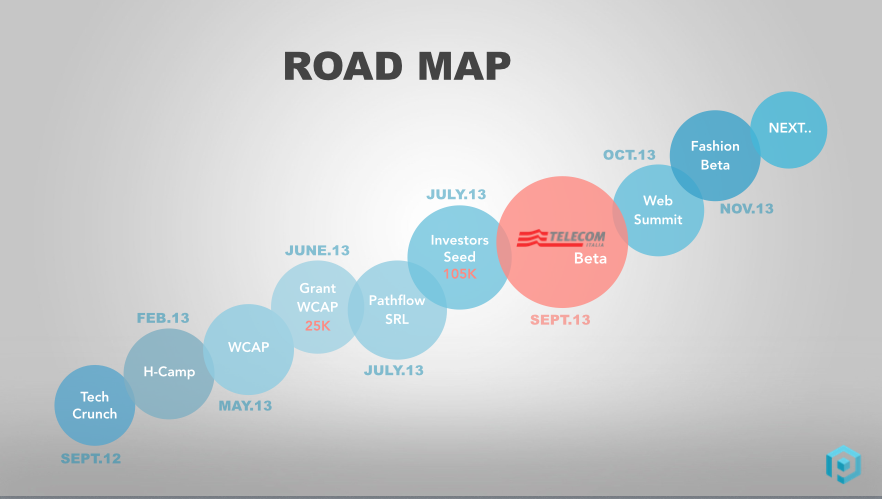
\includegraphics[scale=0.4]{./images/roadmap.png}
\caption{Road Map degli obiettivi raggiunti da Pathflow}
\label{fig:roadmap}
\end{figure}

\subsection{Progetto} \label{ssec:progetto}
Il progetto riguarda la realizzazione di un sistema basato su telecamere per la raccolta di dati di tracciamento all'interno dei retail store. Il sistema ha come fine quello di elaborare statistiche a partire dai dati raccolti. Le statistiche in questione serviranno a fornire alle figure professionali che si occupano del marketing (quali visual merchandiser e marketing manager) la possibilità di migliorare l'esperienza di acquisto del cliente e di ottimizzare i flussi di vendita.\\ \\
Le informazioni verranno raccolte su una piattaforma cloud e rese disponibili agli utilizzatori del sistema tramite delle dashboard, che forniscono dei report e dei grafici che presentano le statistiche in maniera chiara e comprensibile. \\ \\
Dato che il sistema è complesso e vasto nel suo insieme esso è stato diviso in 3 parti:
\begin{itemize}
	\item \textbf{Video Analytics}
	\item \textbf{Back-end Core}
	\item \textbf{Front-end}
\end{itemize}
Il progetto proposto per lo stagista consiste nella realizzazione del modulo di back-end core.\\
Le funzionalità di tale sottosistema comprendono una parte di configurazione del sistema e una parte di generazione statistiche e dati grafici. \\ \\
Nello specifico esso deve permettere l'impostazione dei valori di configurazione delle telecamere, e salvare tali dati in maniera persistente, evitando che vengano perse le opzioni salvate. Tale funzionalità si può suddividere ulteriormente tra vera e propria calibrazione delle telecamere e impostazione di criteri di trasformazione dei dati di tracking (il significato verrà approfondito in seguito). \\
La parte di statistiche comprende la generazione di un \textit{heatmap} della planimetria del locale. Essa a partire dai dati di tracciamento dev'essere in grado di produrre una visualizzazione grafica delle diverse concentrazioni di movimento all'interno dell'area del locale. La planimetria del locale verrà fornita dal cliente in formato vettoriale .DXF. \\ \\Deve essere inoltre in grado di generare alcune statistiche che riguardano: il conteggio delle persone presenti (\textit{counting}), il tempo di attesa davanti alla cassa (\textit{waiting line}), il tempo di ritorno nel locale (\textit{dwell time}), e il tempo trascorso all'interno di alcune aree preimpostate (\textit{bounce rate}).\\

Tale software è inteso per l'utilizzo solo da parte di un utente amministratore (interfaccia grafica molto semplice), che al momento dell'installazione si preoccupa di configurare i dati necessari per il corretto funzionamento del sistema nel suo insieme. Il sistema verrà poi impostato per eseguire periodicamente il trasferimento dei dati generati nel server locale (quello che risiede nello store) verso il server cloud.
Il software dovrà funzionare sulle principali piattaforme (Mac OS/Linux/Windows).















